\documentclass[12pt]{article}
\usepackage{graphicx} % Required for inserting images
\graphicspath{ {./montageImages/} }

\title{montages \& technicalities}
\author{Annabelle Chan}
\date{October 2024}

\begin{document}
\maketitle
Link: https://www.learningeeg.com/montages-and-technical-components

Author: David Valentine, MD

Date: 2020

\section{The 10-20 System} 
Standard placement of the electrodes (splits the skull in to increments of 10 percent or 20 percent to place the electrodes). This ensures each electrode is relatively positioned to all the others and making it possible for every EEG study to be consistent despite a person’s head shape and size. Each electrode is identified with a letter and a number. Each letter corresponding to its region of the brain: F Frontal, T Temporal, P Parietal, and O Optical). Exceptions are F7 and F8, both of which are over the anterior temporal region. The number corresponds to the side of the brain (odds on the left and evens on the right) and the particular area for each region. For the midline/central electrodes, the number is replaced with z
Example:
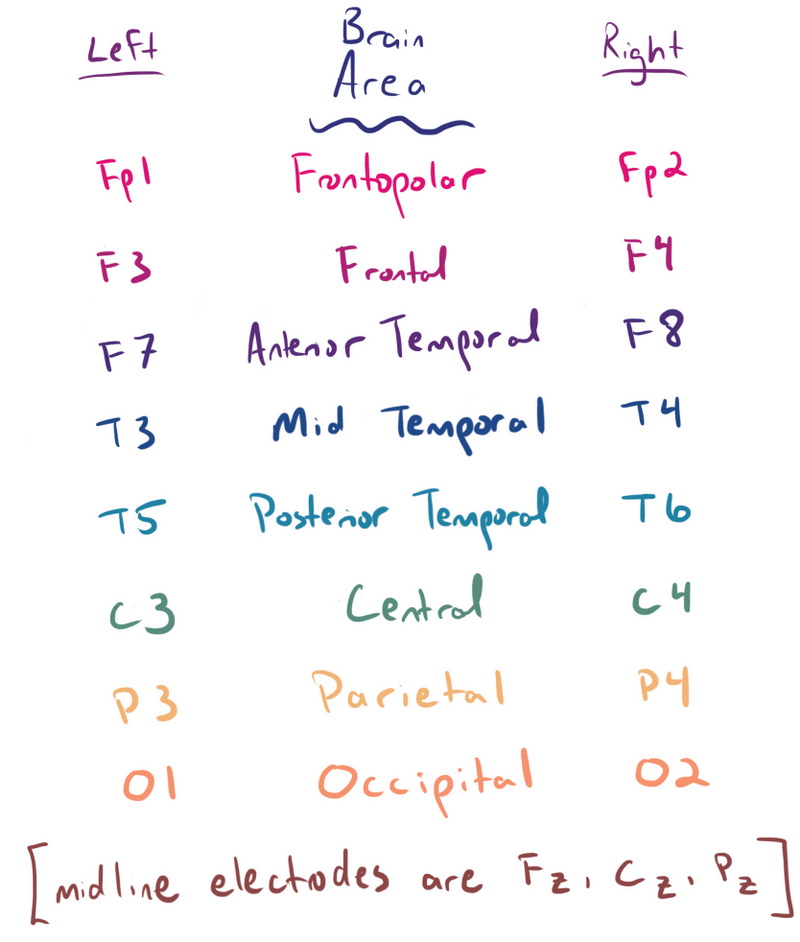
\includegraphics[scale=0.4]{montage1020system1}
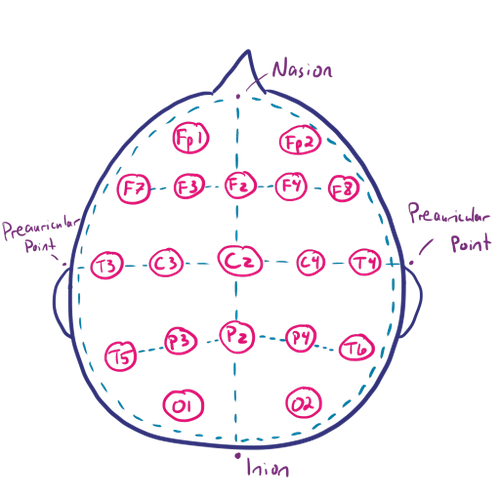
\includegraphics[scale=0.4]{montage1020system2}

Setup for standard electrodes
1) Find the nasion (the top of the nose bridge, between the eyes) and the inion (the small bump in the middle of the back of the head).
2) Divide the head into consecutive increments of 10\% and 20\% to find the placement of the electrodes

Special electrodes:
Subtemporal electrodes (T1 and T2) provide more information about the anterolateral temporal region.
A1 and A2 electrodes (or M1 and M2) are placed on the auricle of the ear for referential montages.
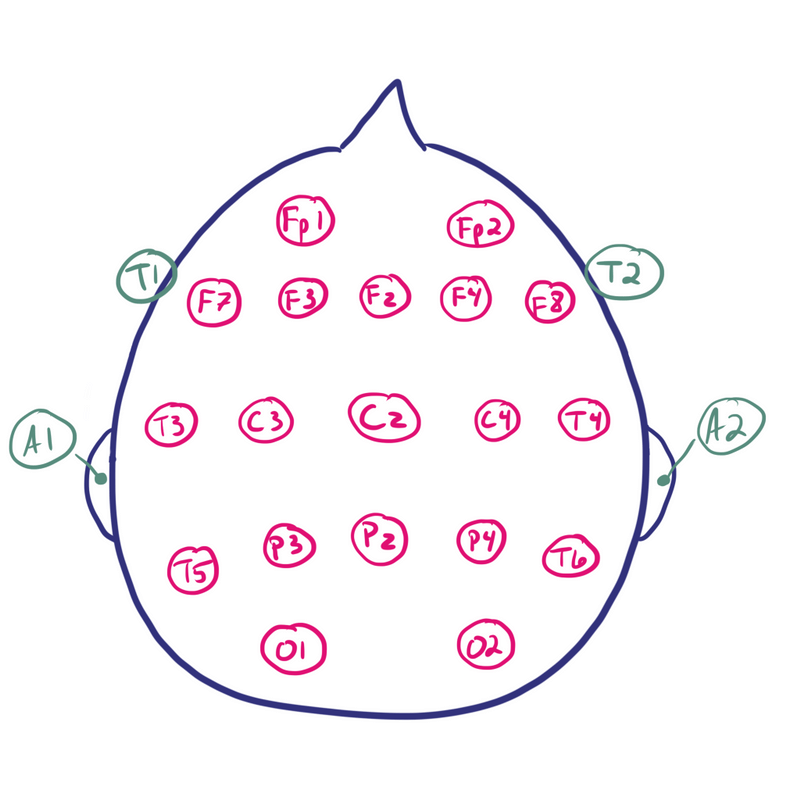
\includegraphics[scale=0.4]{montage1020system3}

\section{Bipolar montage} 
For a bipolar montage, each electrode’s voltage is linked and compared to an adjacent one to form a chain of electrodes.

Double banana (most common bipolar montage): each electrode is linked and compared to the one behind it (e.g. Fp2 is compared to F8, F8 is compared to T4, etc.) 
Two chains per side-Outside temporal chain, and inside parasagittal chain-and the central train 

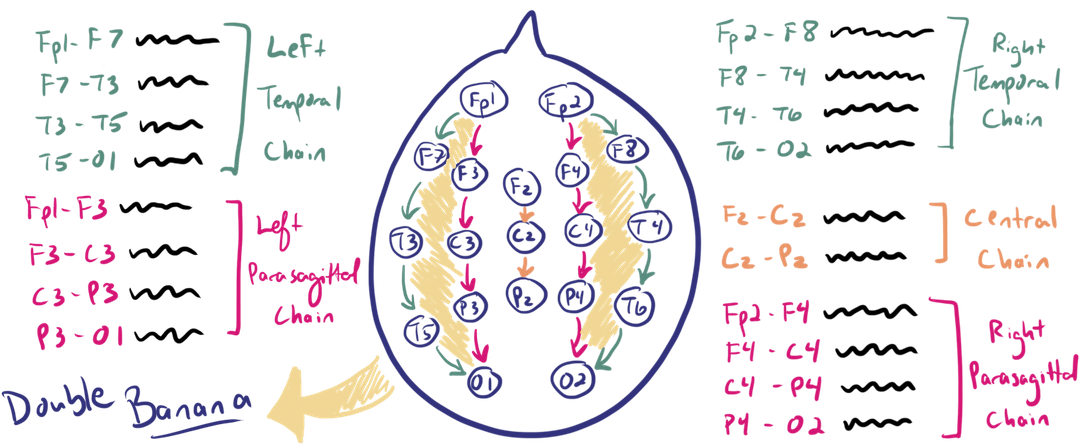
\includegraphics[scale=0.4]{doubleBanana}

In each chain, an electrode’s voltage is compared to that of the electrode behind it, so each tracing line is a pair of electrodes in which the voltage of the second electrode is subtracted from the voltage of the first 
If the first electrode in the tracing line is more positive/higher than the second, you get a positive, downward deflection
If the second electrode is more positive/higher, you get a negative, upward deflection
The article contains step by step images 
Phase reversal: the closest electrode to a nearby discharge sees the greatest voltage and the other electrode tracings “point” towards the closest electrode to a nearby discharge on the tracing.
The middle electrode of the pair that makes the reversal is the electrode of maximal voltage.
Negative discharges cause the surrounding tracings to point toward the electrode of maximal voltage
Positive discharges cause the surrounding tracings to point away from the electrode of max voltage 
Generally negative phase reversals are seen with epileptiform activity and positive ones are seen with various artifacts
Negative phase reversals move towards one another and positive phase reversals more away from each other
End of chain phenomenon: you only see half of any possible phase reversals at these electrodes because for the first electrode in each chain there is not an electrode in front to compare it to, and the last electrodes don’t have one behind them to compare to
Bipolar circumferential montage: the electrodes are linked not in an anterior to posterior chain but in a circle around the head
No end of chain phenomenon because the all electrodes in the chain have a point of comparison 
Does not include much of middle regions/parasagittal electrodes so this montage shouldn’t be used to screen tracings but only to clarify particular discharges 
Bipolar TI-T2 montage: similar to the double banana but places the parasagittal chains on top and includes the subtemporal T1 and T2 electrodes. Suffers from end of chain issue.
Transverse montage: makes chains not front to back but side to side. Helps lateralize activity if the dominant hemisphere for a discharge is unclear on double banana
Referential montage 
Useful to clarify the point of maximal electronegativity if it remains unclear on a bipolar view.
Compares all of the electrodes to single reference point (usually the average of the voltage of all electrodes, average montage, or the electricity silent auricle of the ear)
Every wave that goes up is negative and every wave that goes down is positive. 
There are no phase reversals so the highest amplitude waveform is the one with the greatest voltage (downward or upward)
Makes it easier to find the point of maximal voltage in a tracing but makes it harder to see epileptiform discharges when screening (no phase reversal to stand out from the background)
Page speed
Reading speed determines how many seconds of the study are displayed across your computer at one time. 
The standard adult reading speed is 30 mm/sec and the standard neonatal speed is 15 mm/sec
The higher your reading speed the fewer seconds displayed on your screen at a time, and the more stretched out the waves appear
EEG tracings used to be recorded by ink nibs fluctuating on a continuously scrolling ream of paper. 
The ink nibs fluctuate at the same speed for any speed of the paper as they recorded the electrophysiologic signal.
The more mm the paper moved per second, the more drawn out each second of tracing was
Sensitivity 
The higher the number the lower the sensitivity (same reasoning as page speed)
The higher numbers for sensitivity lead to smaller appearing waveforms
\end{document}